%!TEX root = ../thesis.tex
% ******************************* Thesis Appendix A ****************************
\chapter{Resultados finales}\label{anex:results}

\begin{figure}
\begin{center}
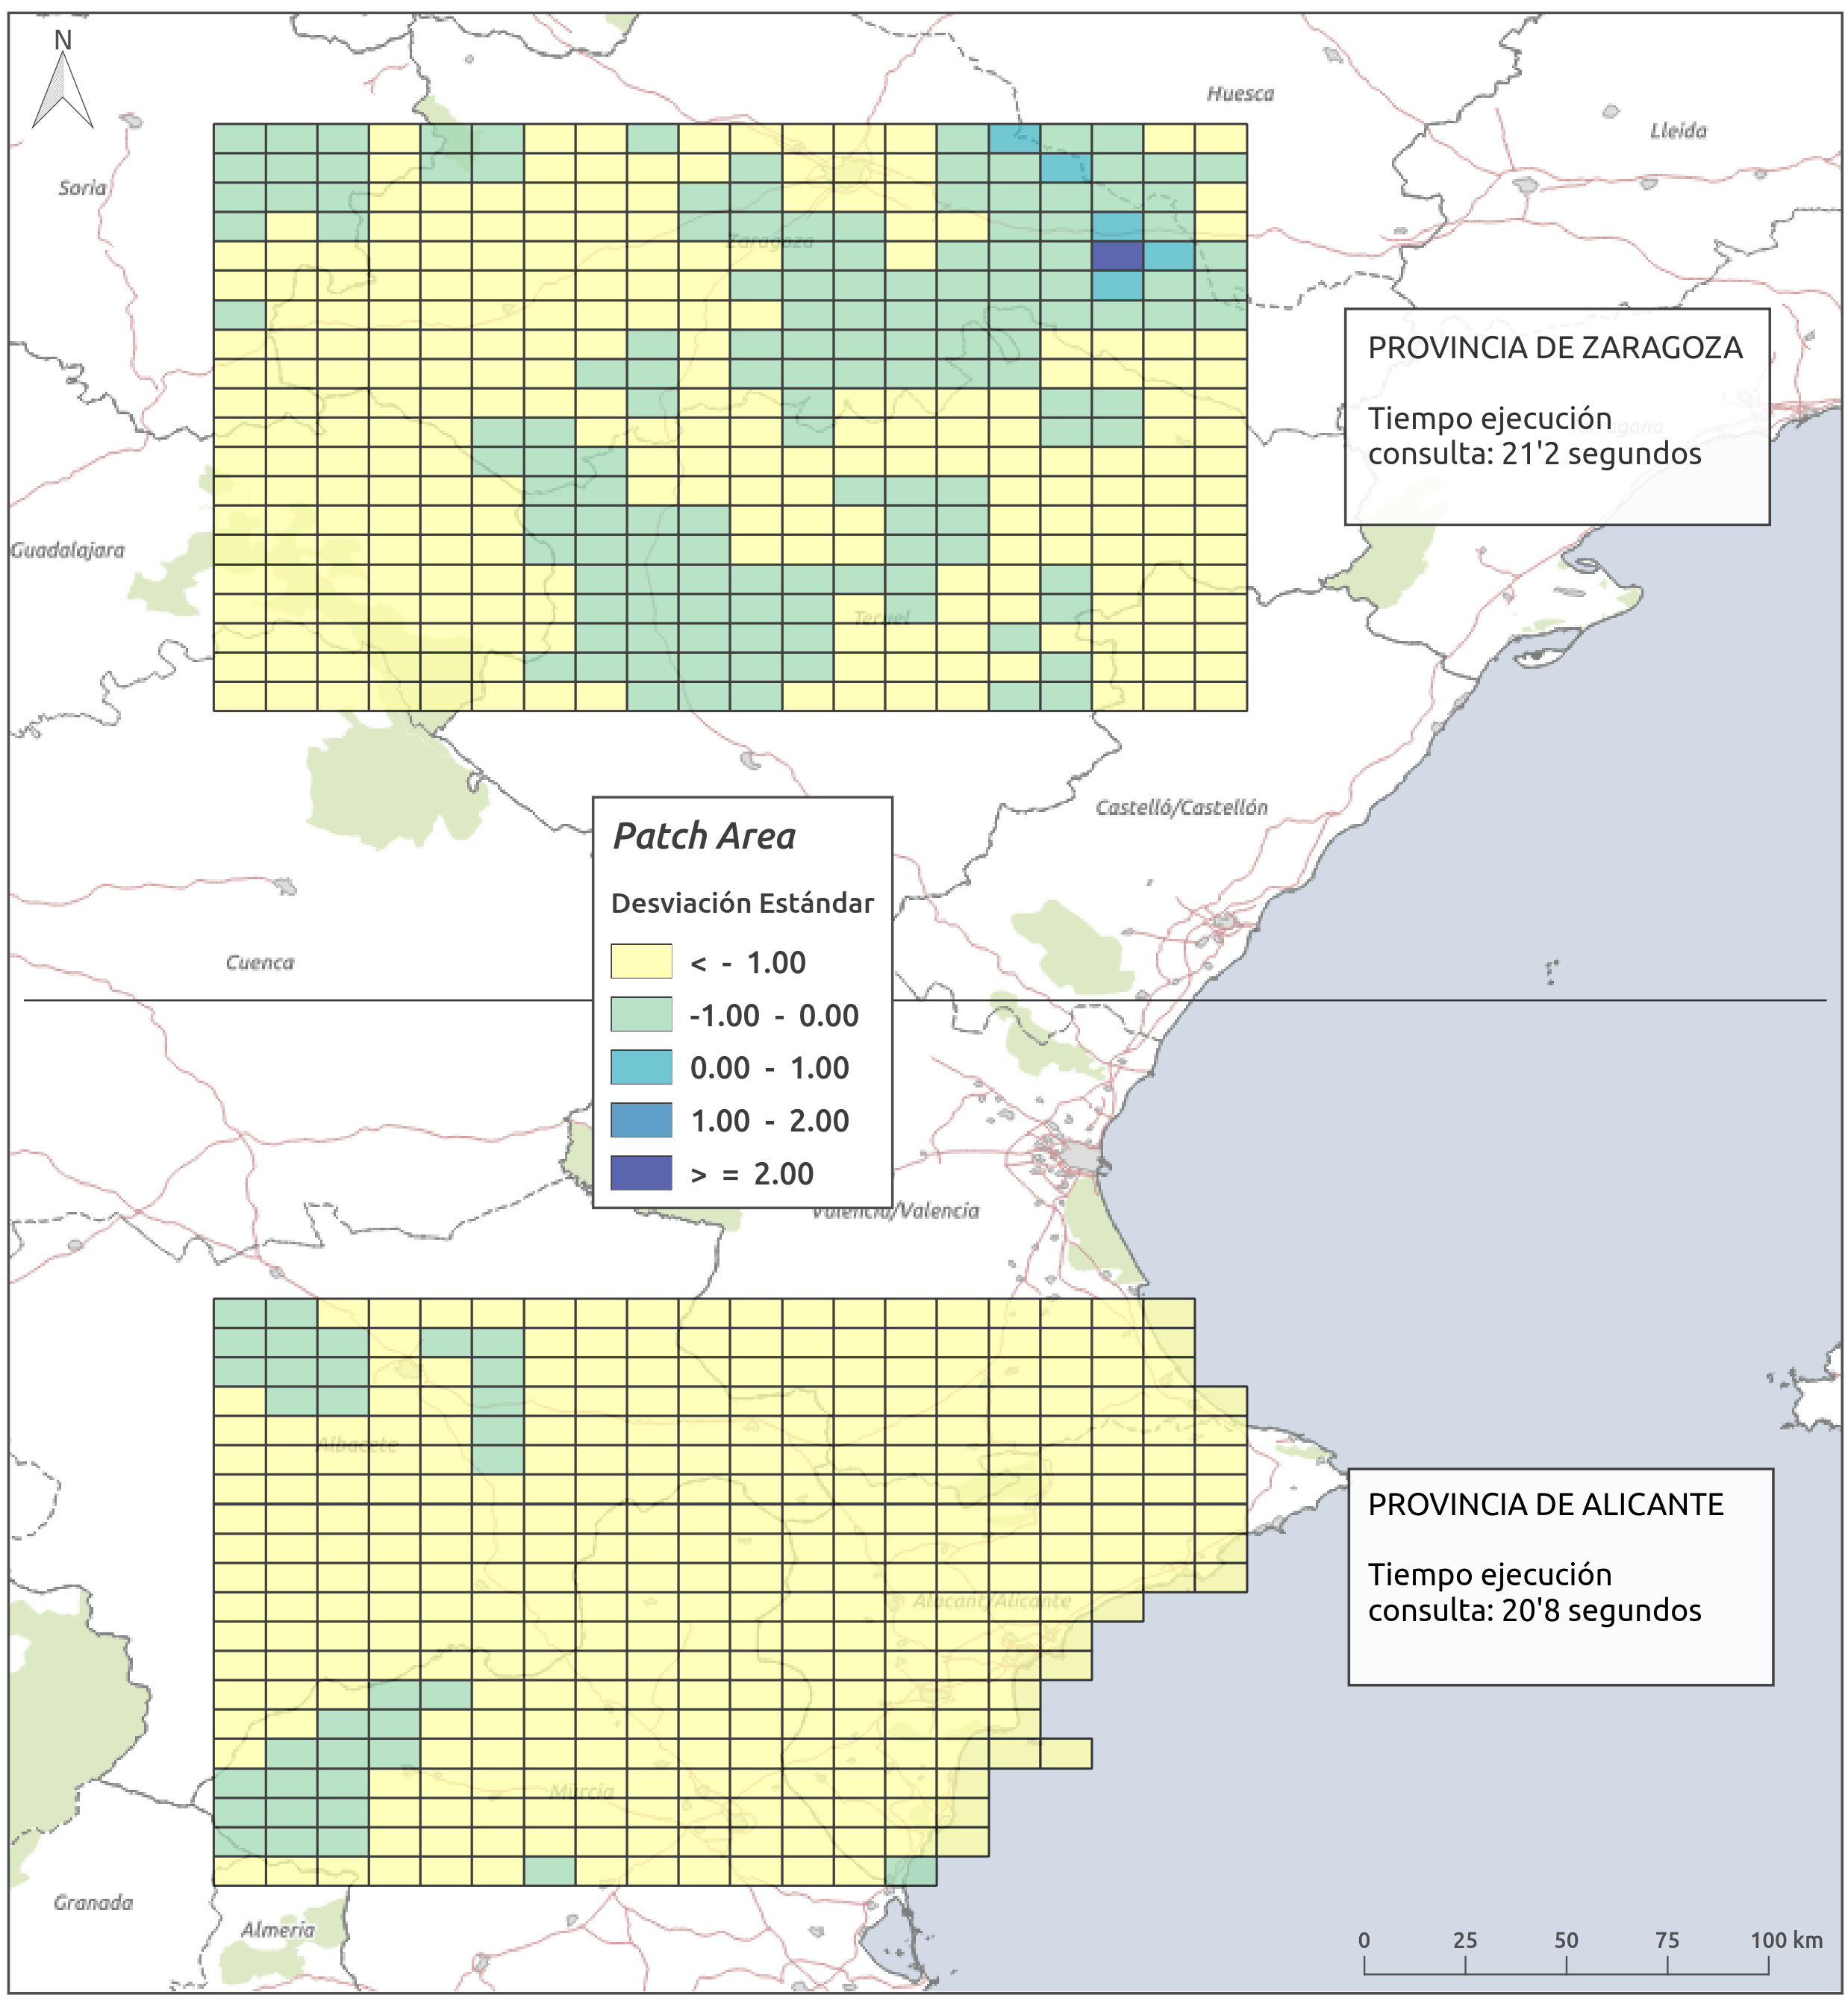
\includegraphics[width=\textwidth]{ResultadosyDiscusion/Figs/Results/p_25.png}
\caption{Título. \label{fig:p_25}}
\end{center}
\end{figure}

\begin{figure}
\begin{center}
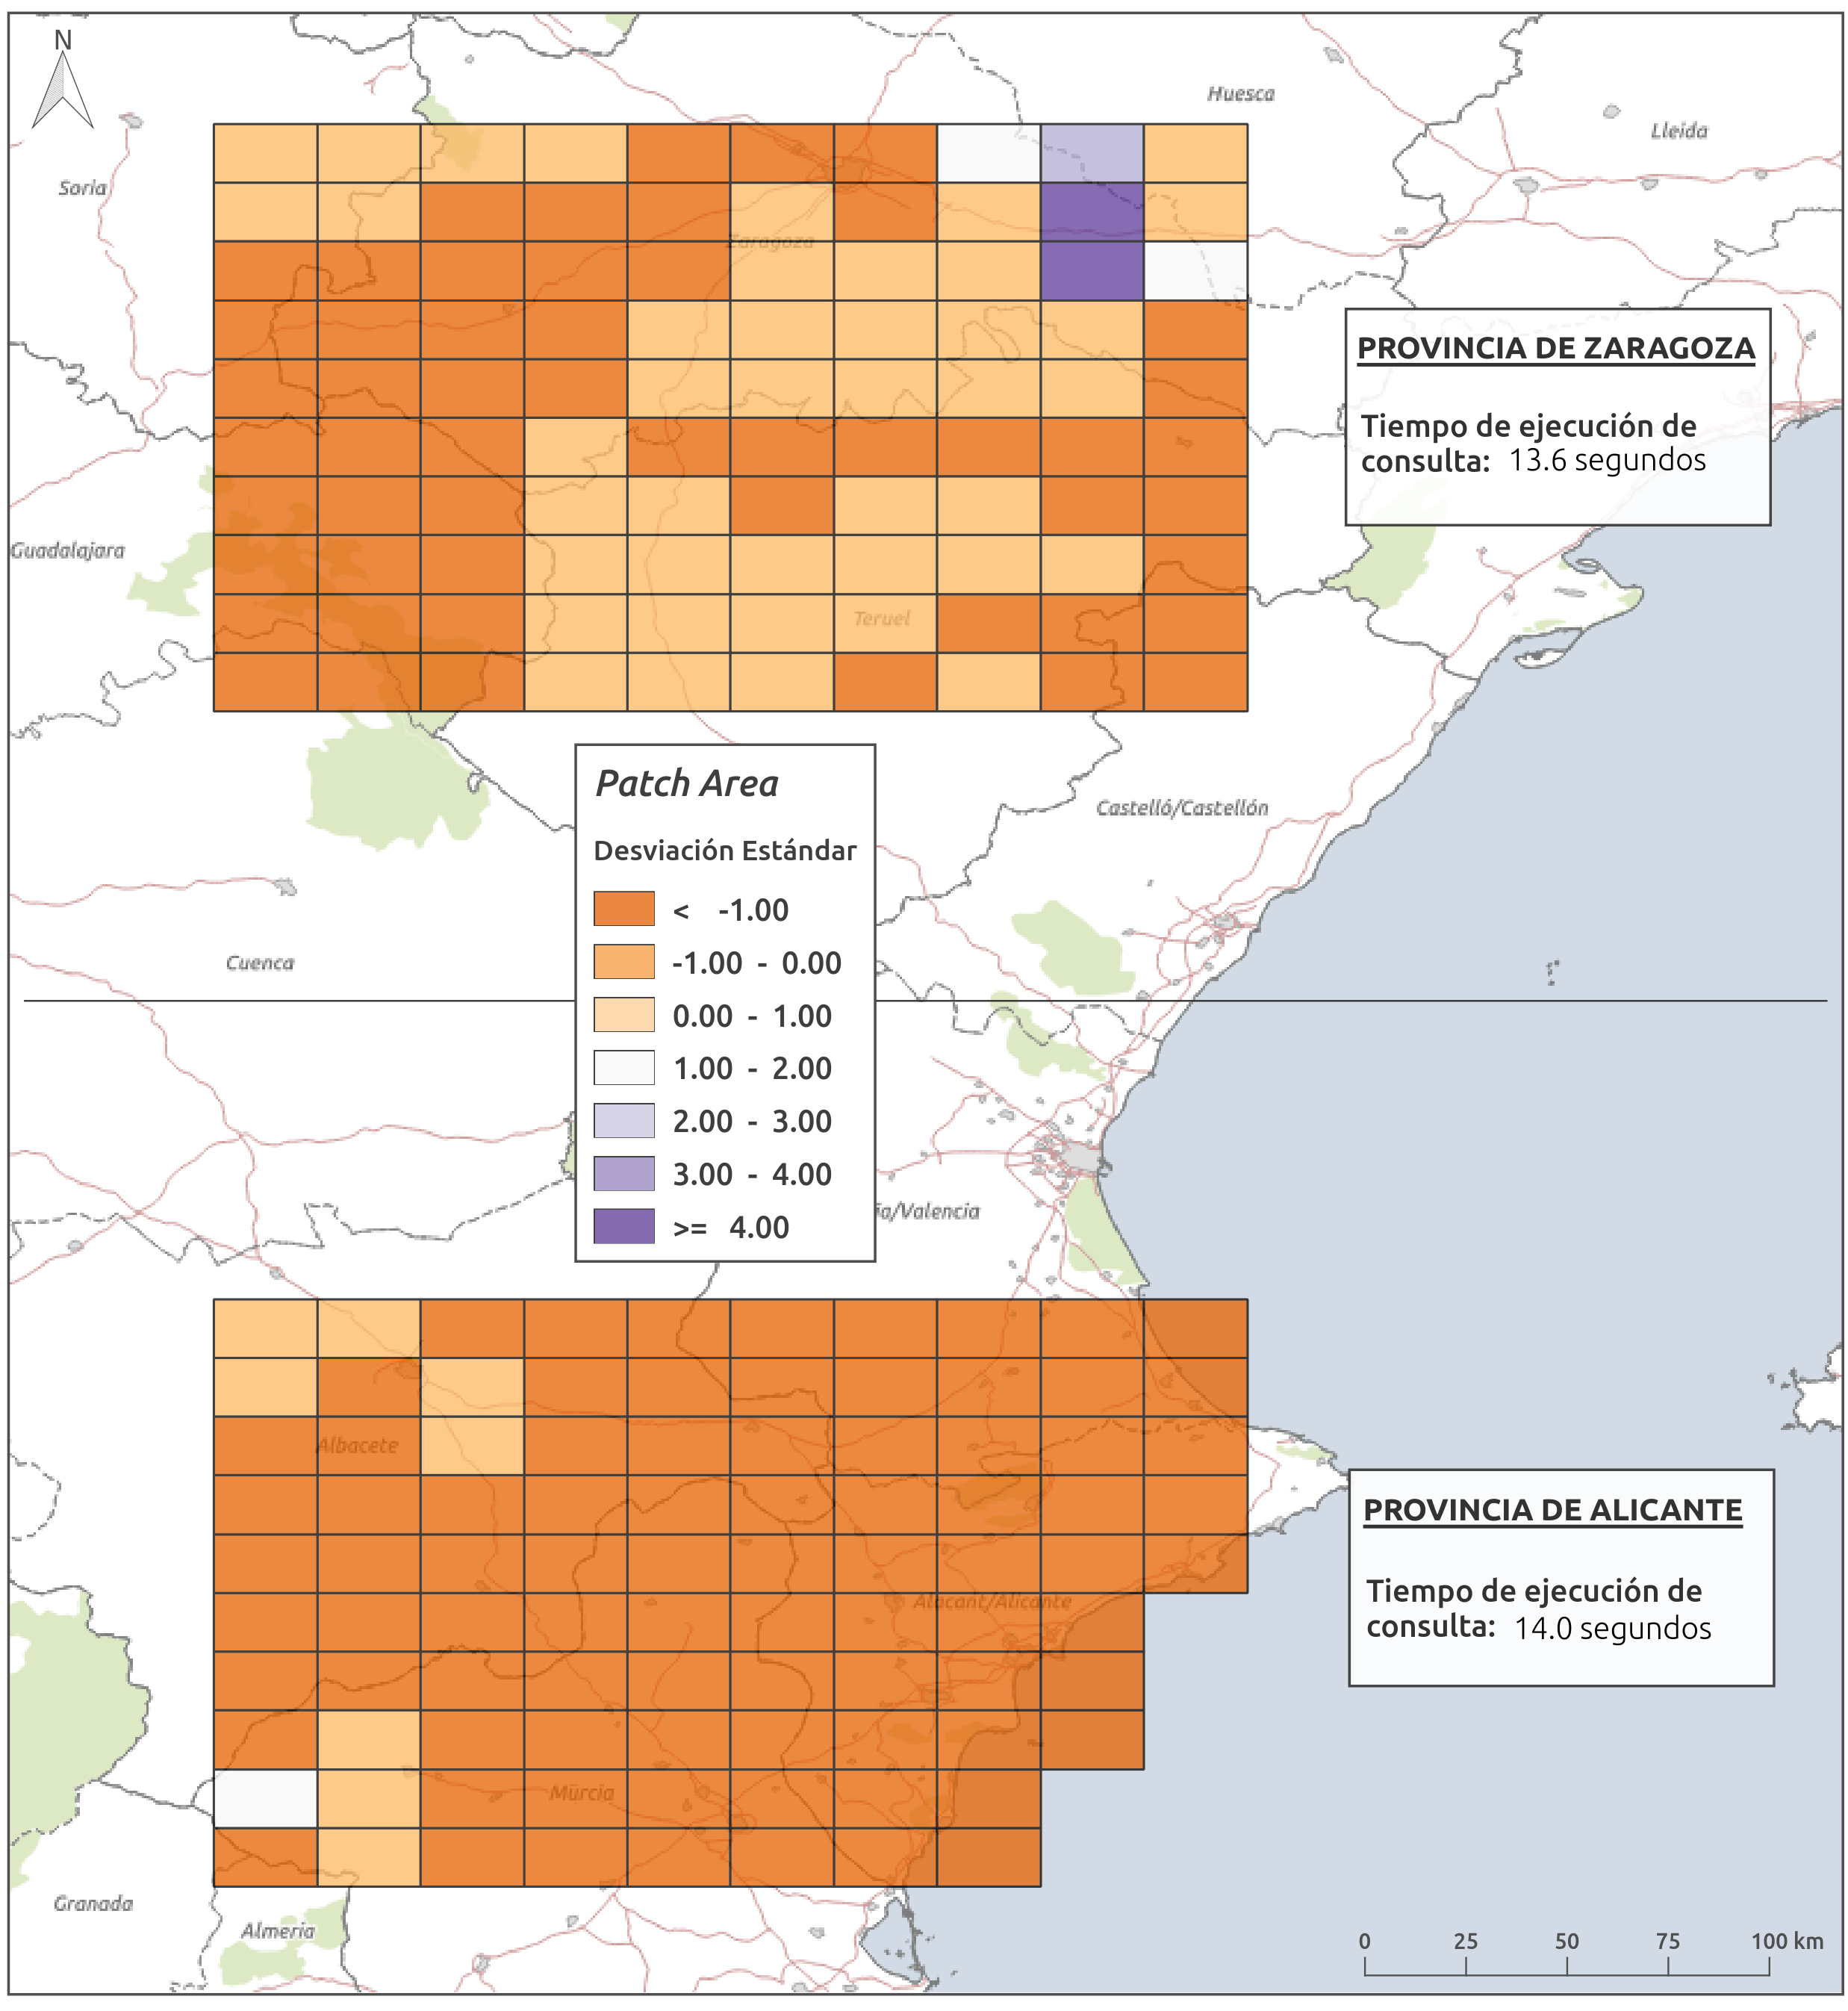
\includegraphics[width=\textwidth]{ResultadosyDiscusion/Figs/Results/p_50.png}
\caption{Título. \label{fig:p_50}}
\end{center}
\end{figure}

\begin{figure}
\begin{center}
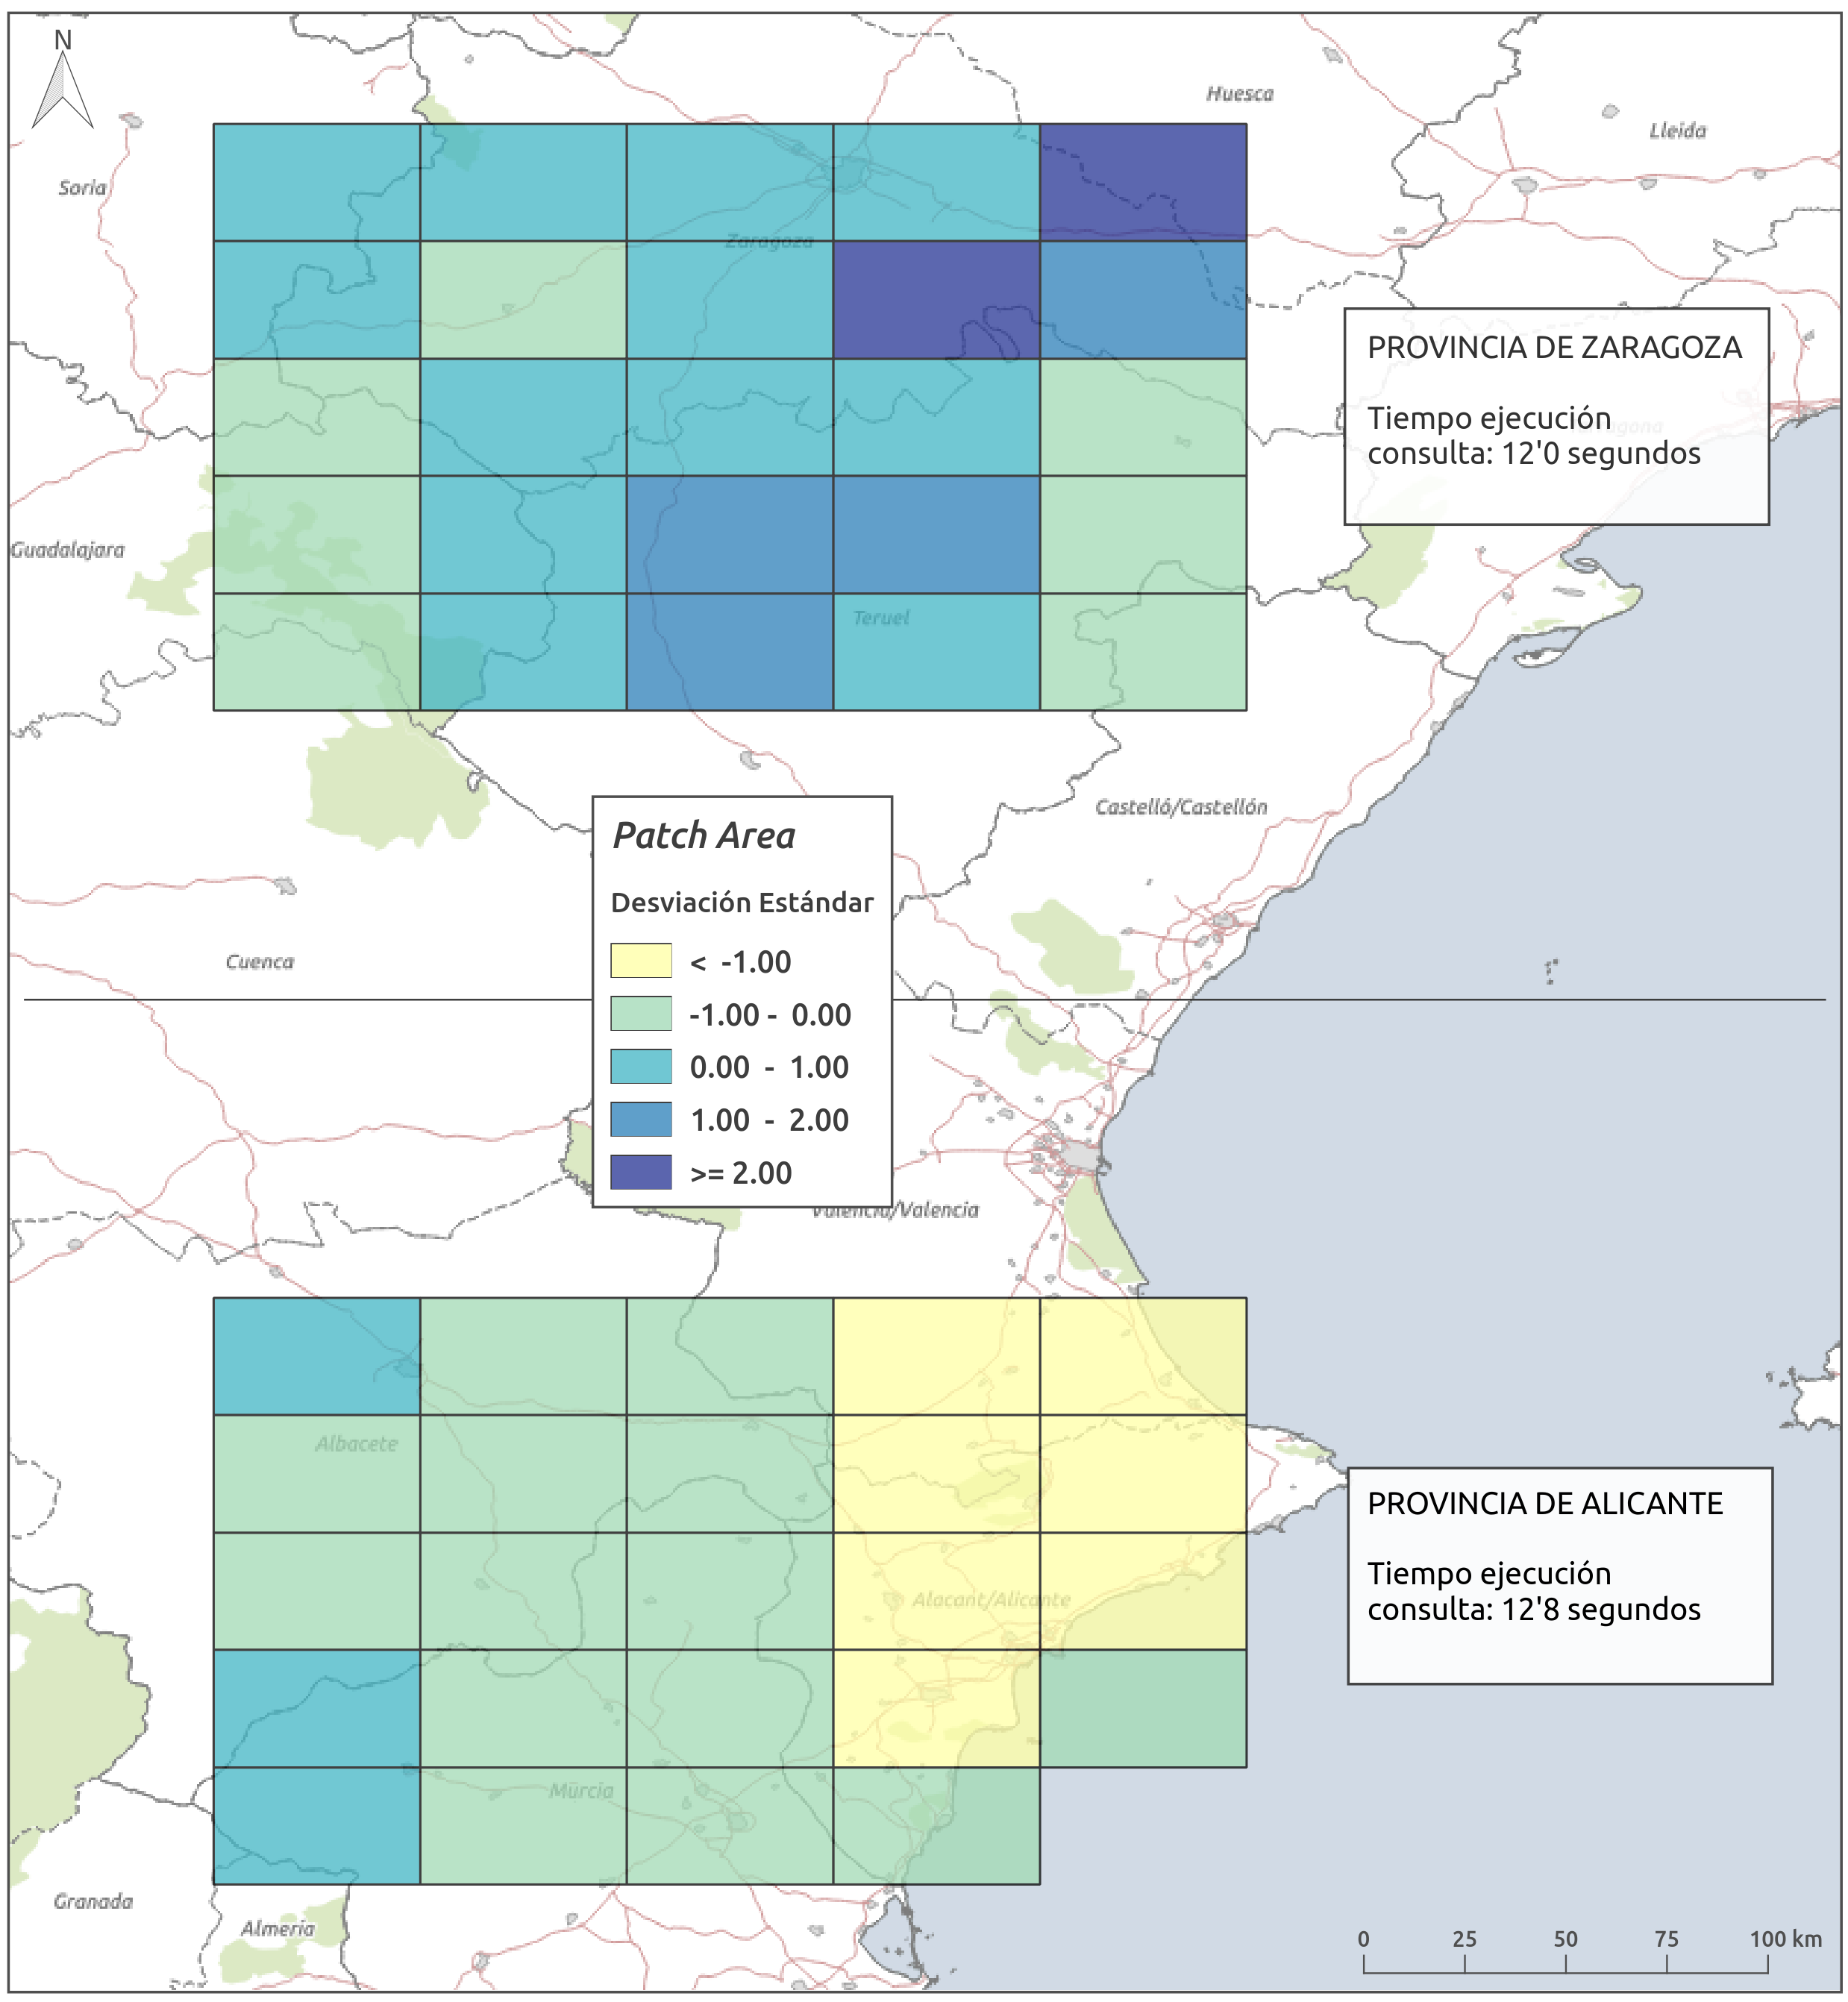
\includegraphics[width=\textwidth]{ResultadosyDiscusion/Figs/Results/p_100.png}
\caption{Título. \label{fig:p_100}}
\end{center}
\end{figure}

\begin{figure}
\begin{center}
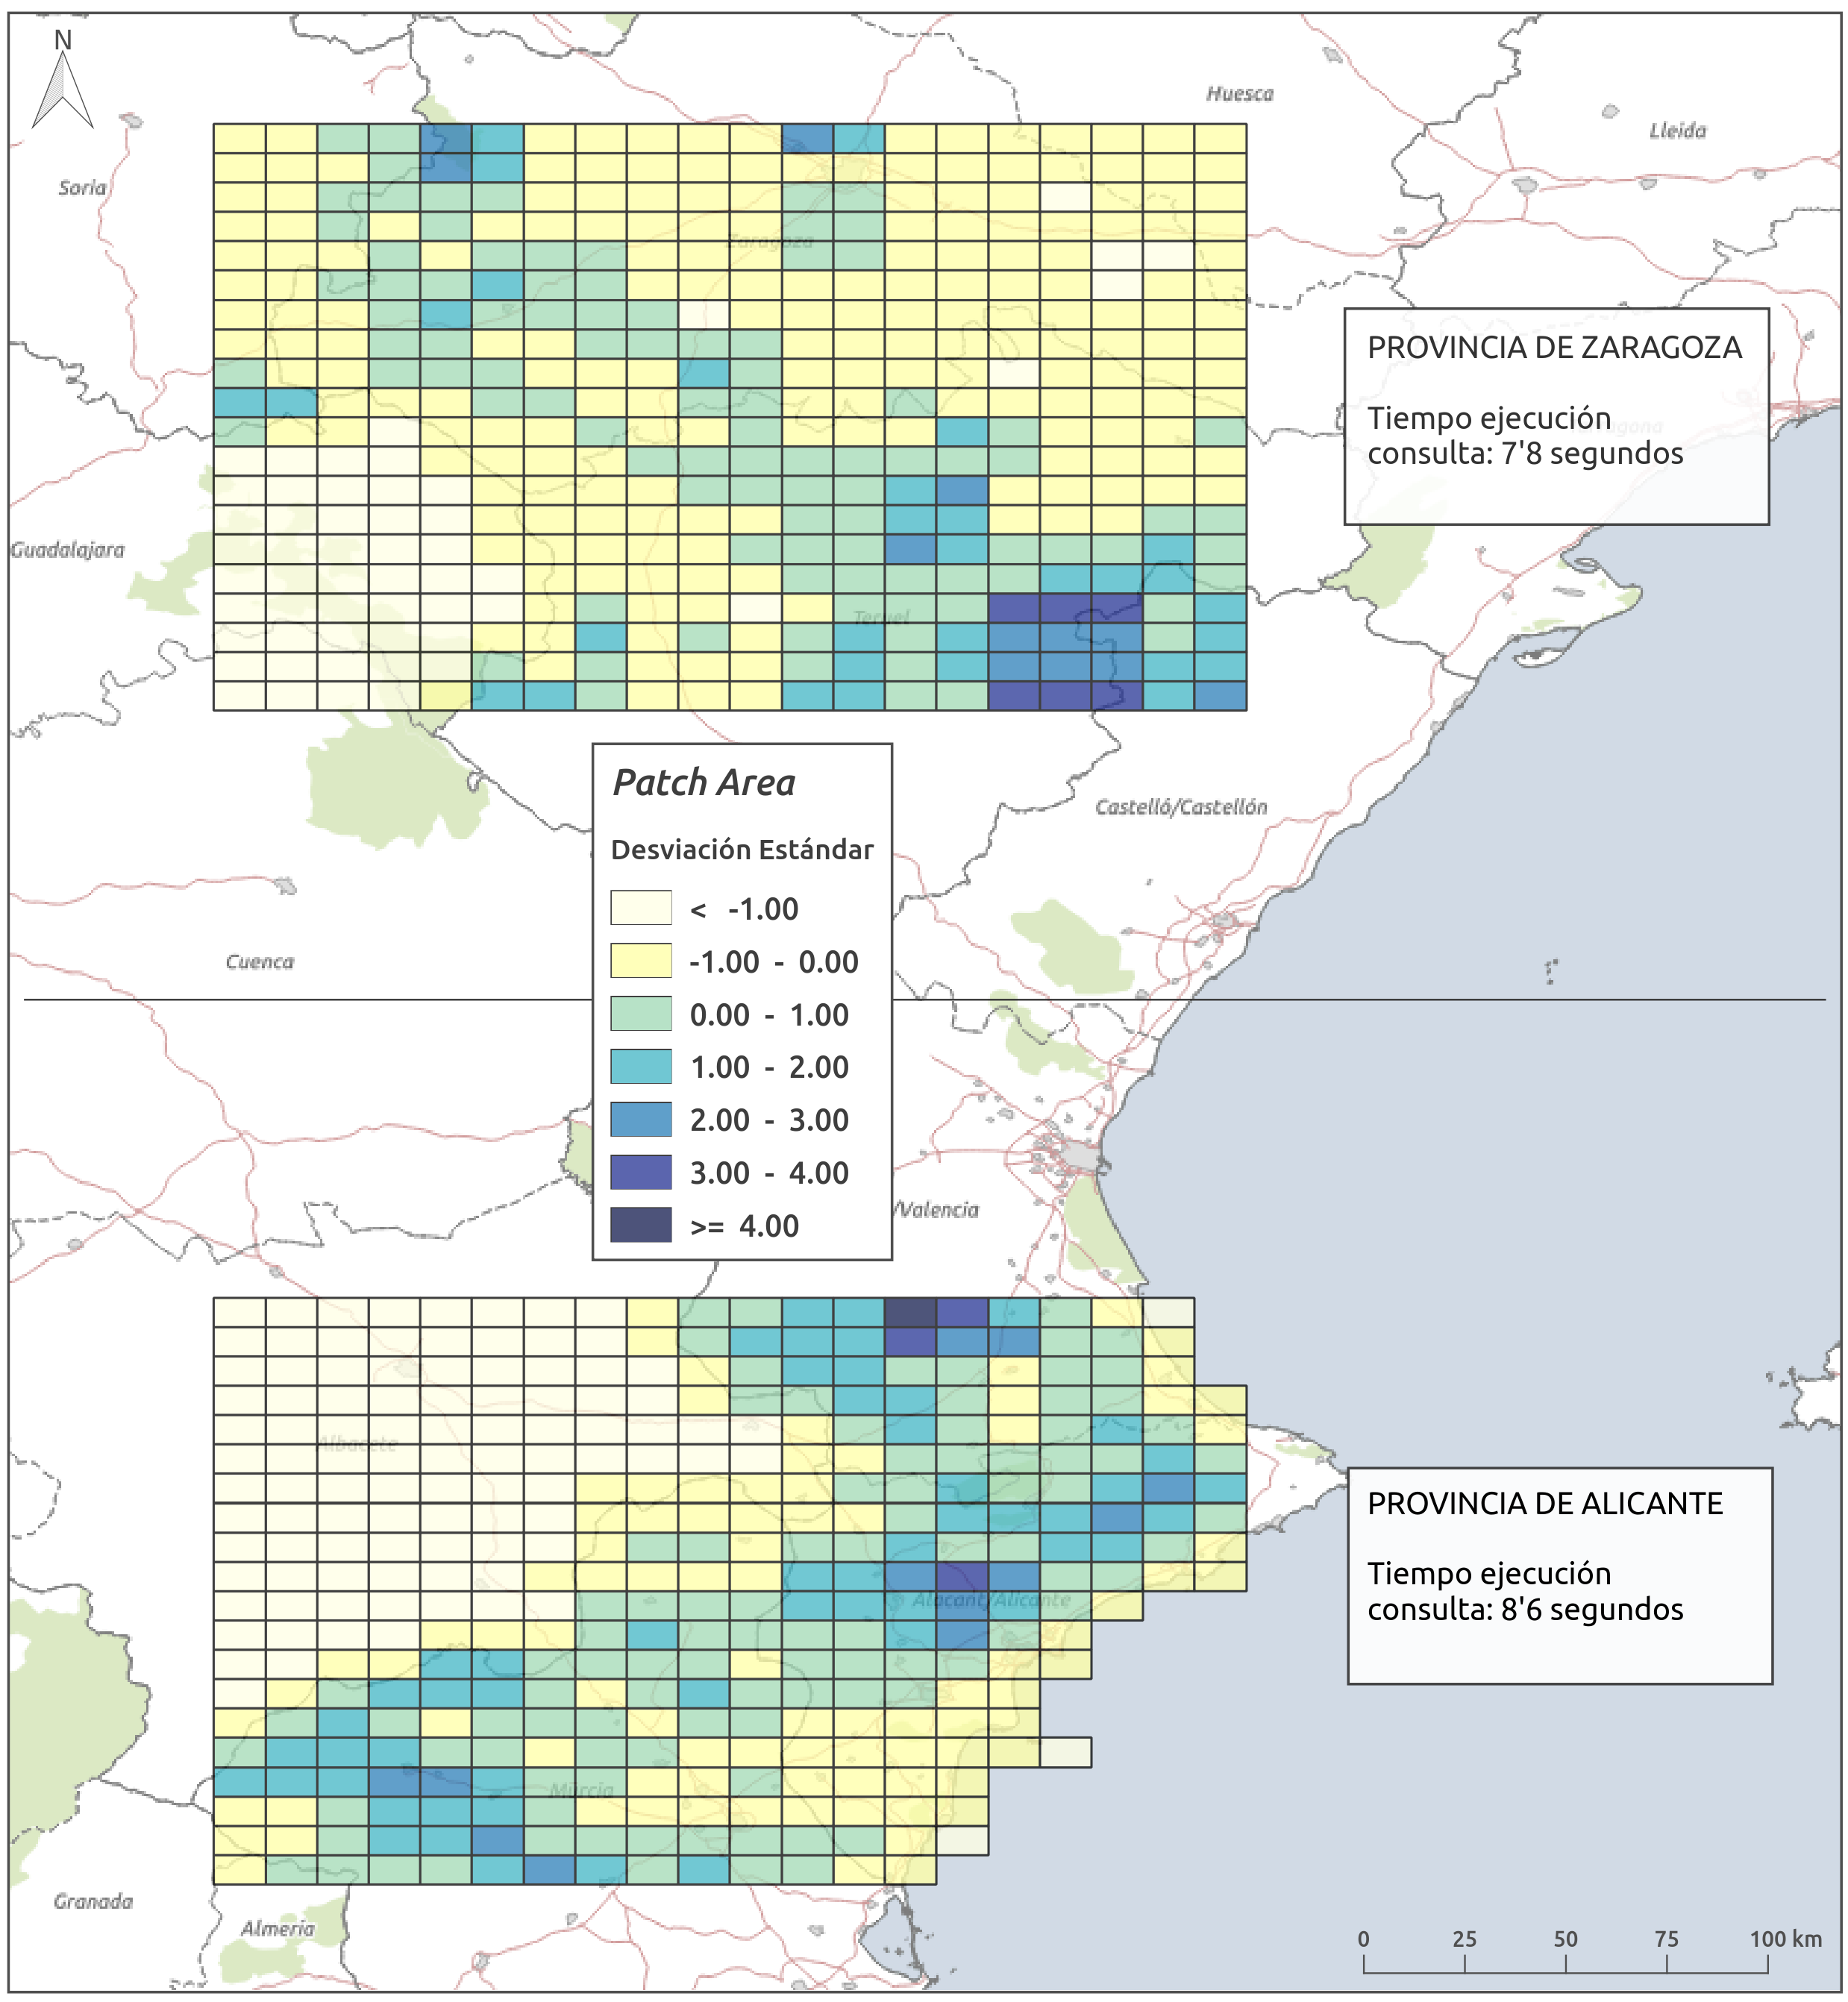
\includegraphics[width=\textwidth]{ResultadosyDiscusion/Figs/Results/c_25.png}
\caption{Título. \label{fig:c_25}}
\end{center}
\end{figure}

\begin{figure}
\begin{center}
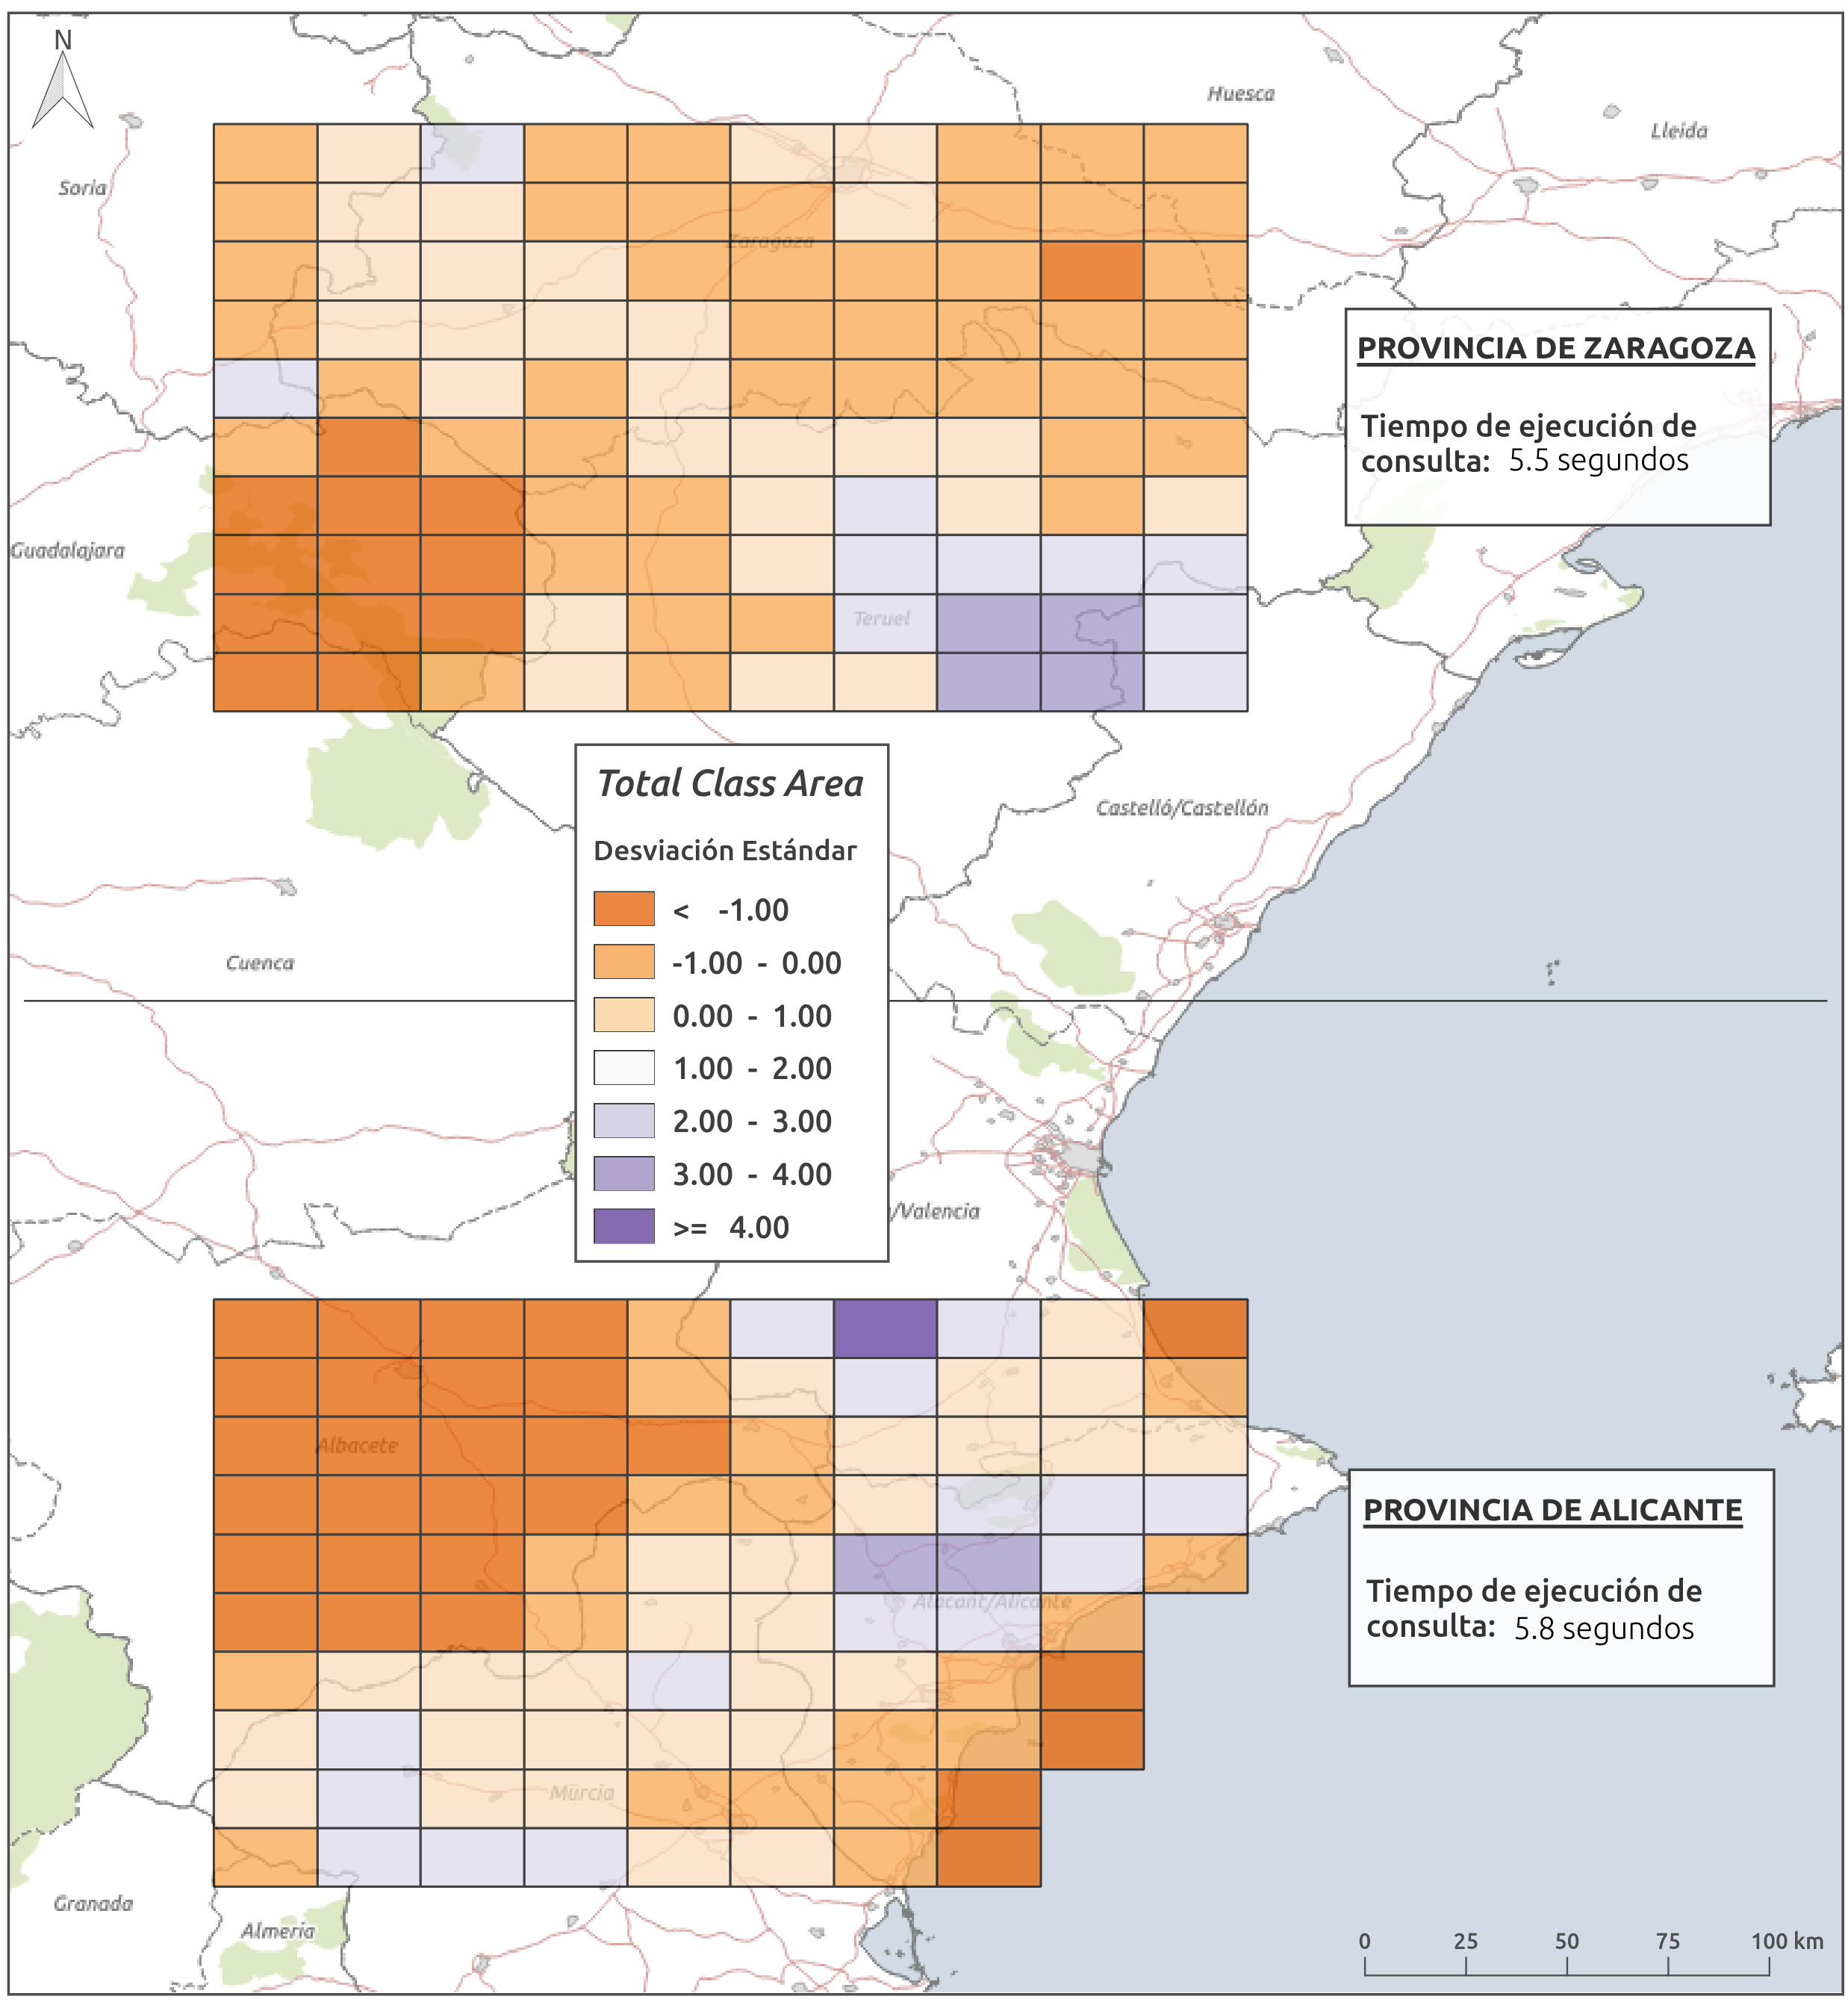
\includegraphics[width=\textwidth]{ResultadosyDiscusion/Figs/Results/c_50.png}
\caption{Título. \label{fig:c_50}}
\end{center}
\end{figure}

\begin{figure}
\begin{center}
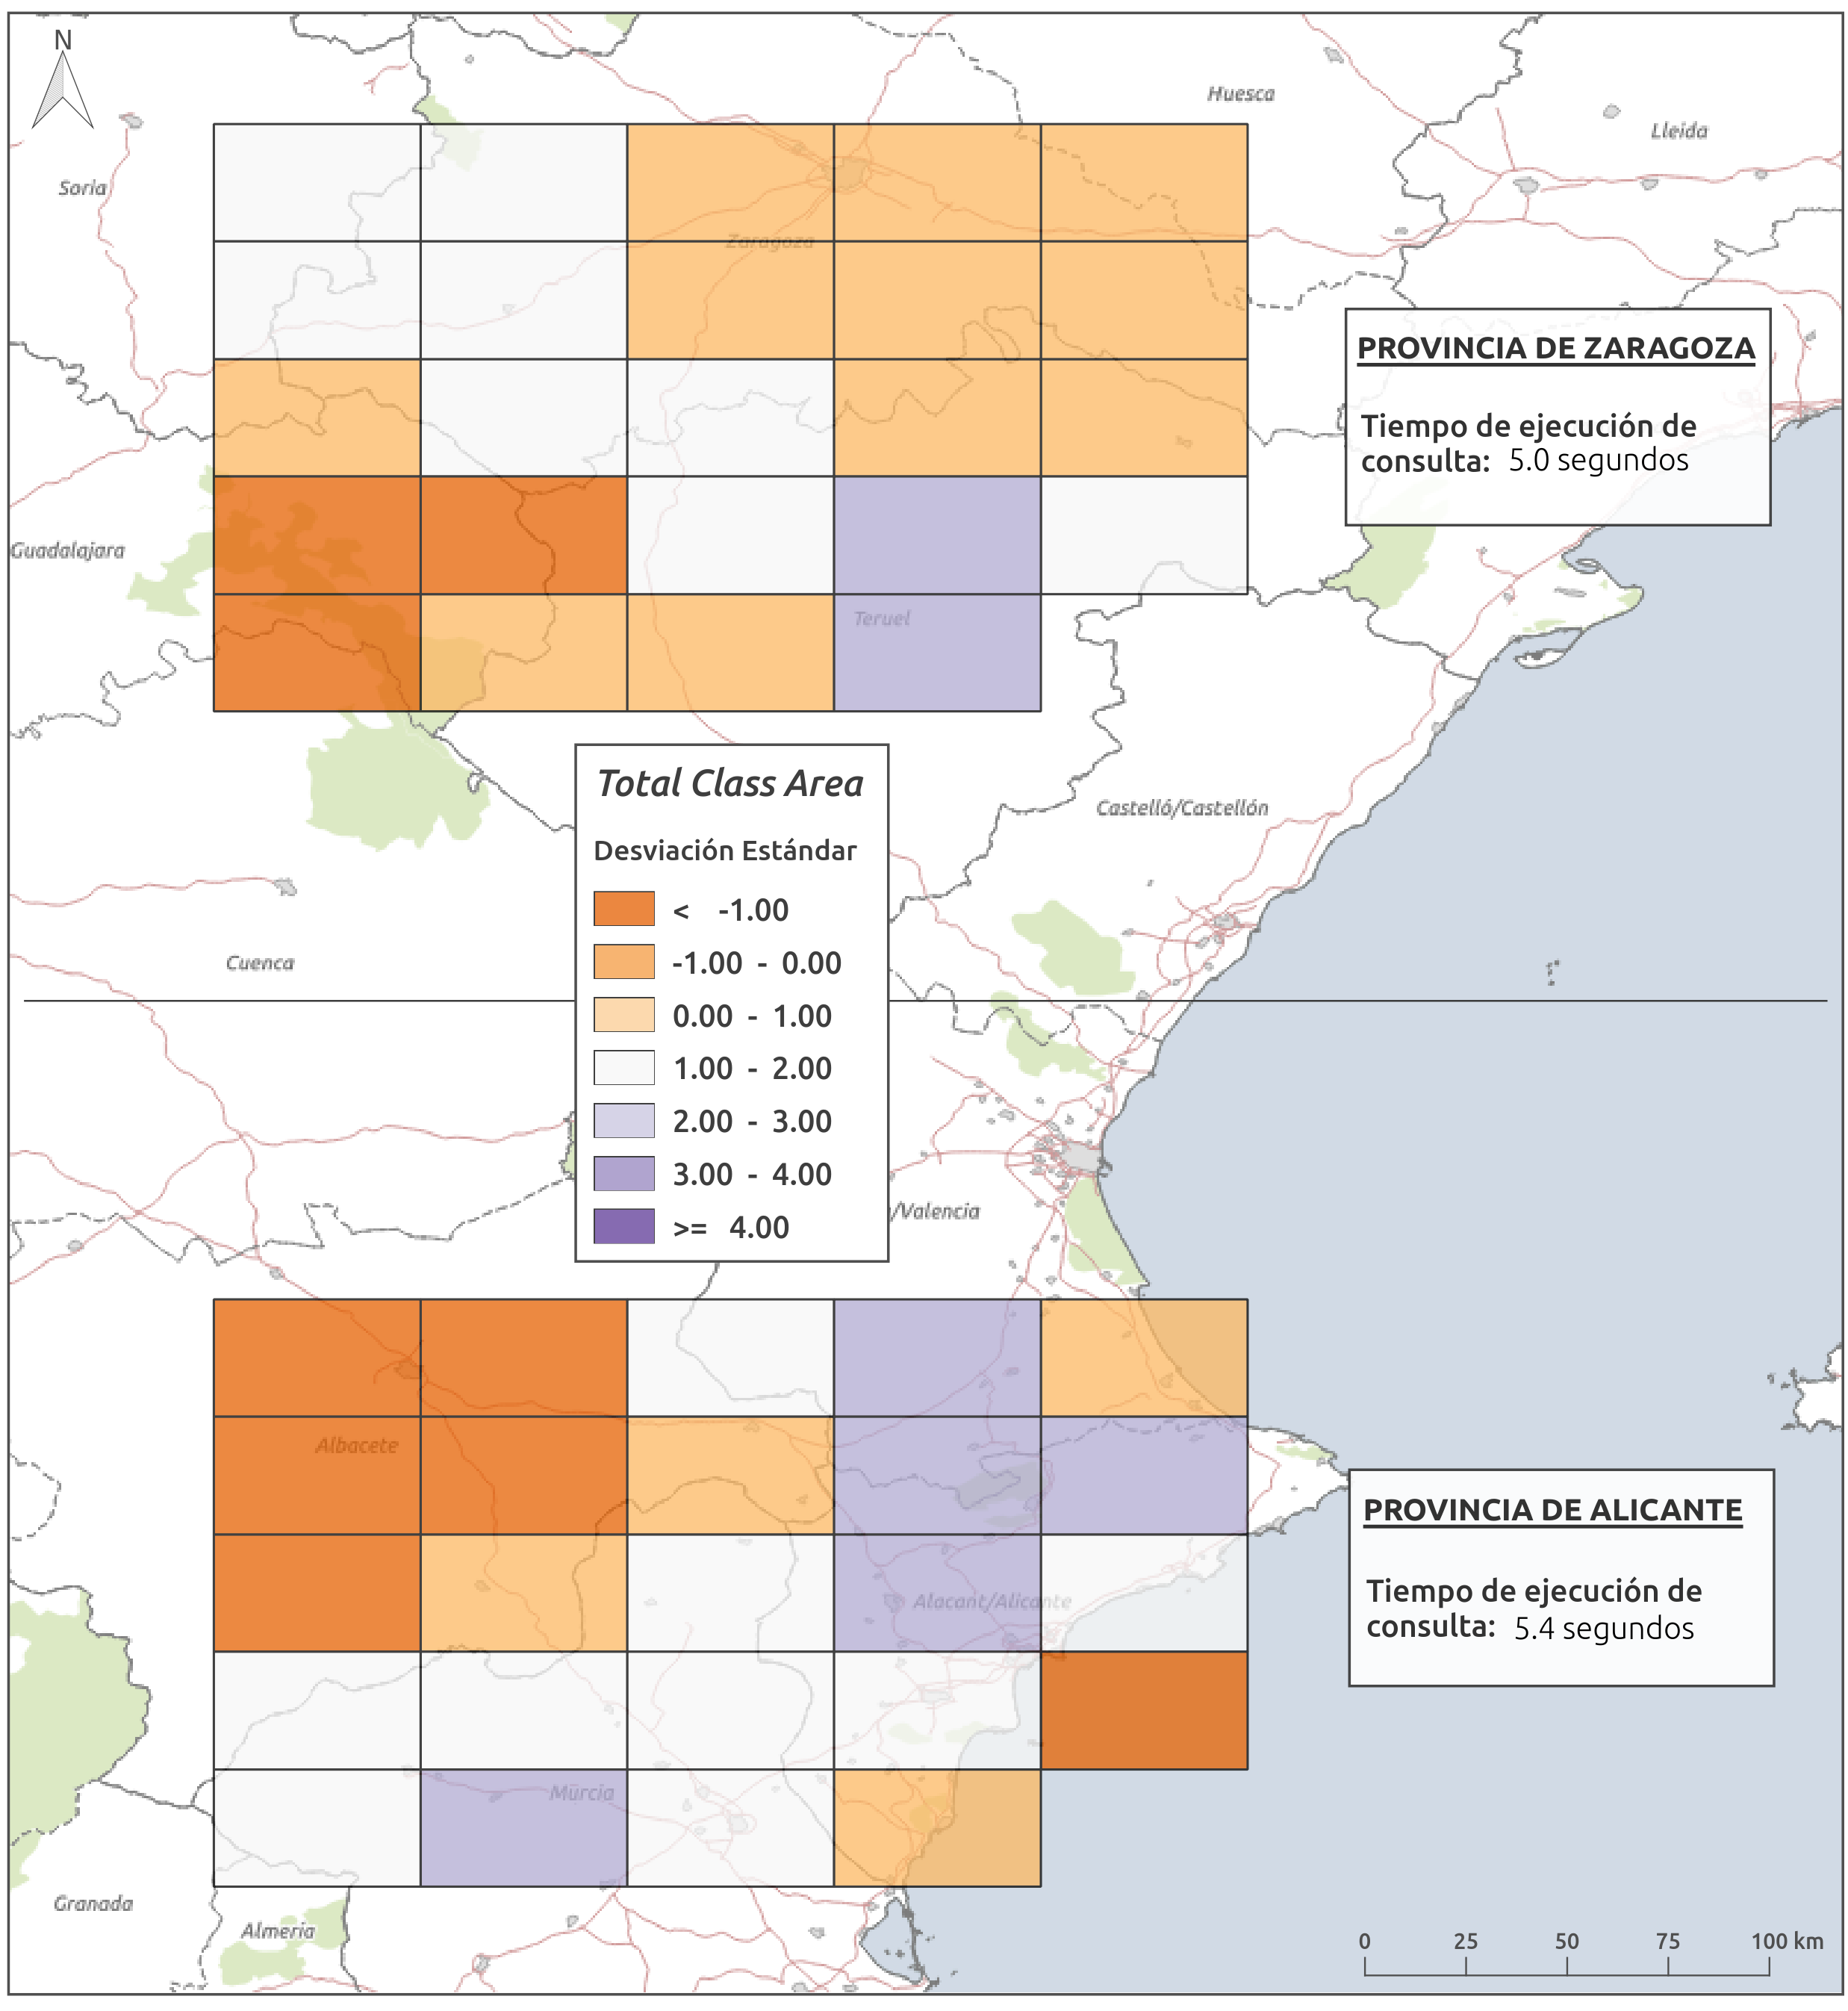
\includegraphics[width=\textwidth]{ResultadosyDiscusion/Figs/Results/c_100.png}
\caption{Título. \label{fig:c_100}}
\end{center}
\end{figure}

\begin{figure}
\begin{center}
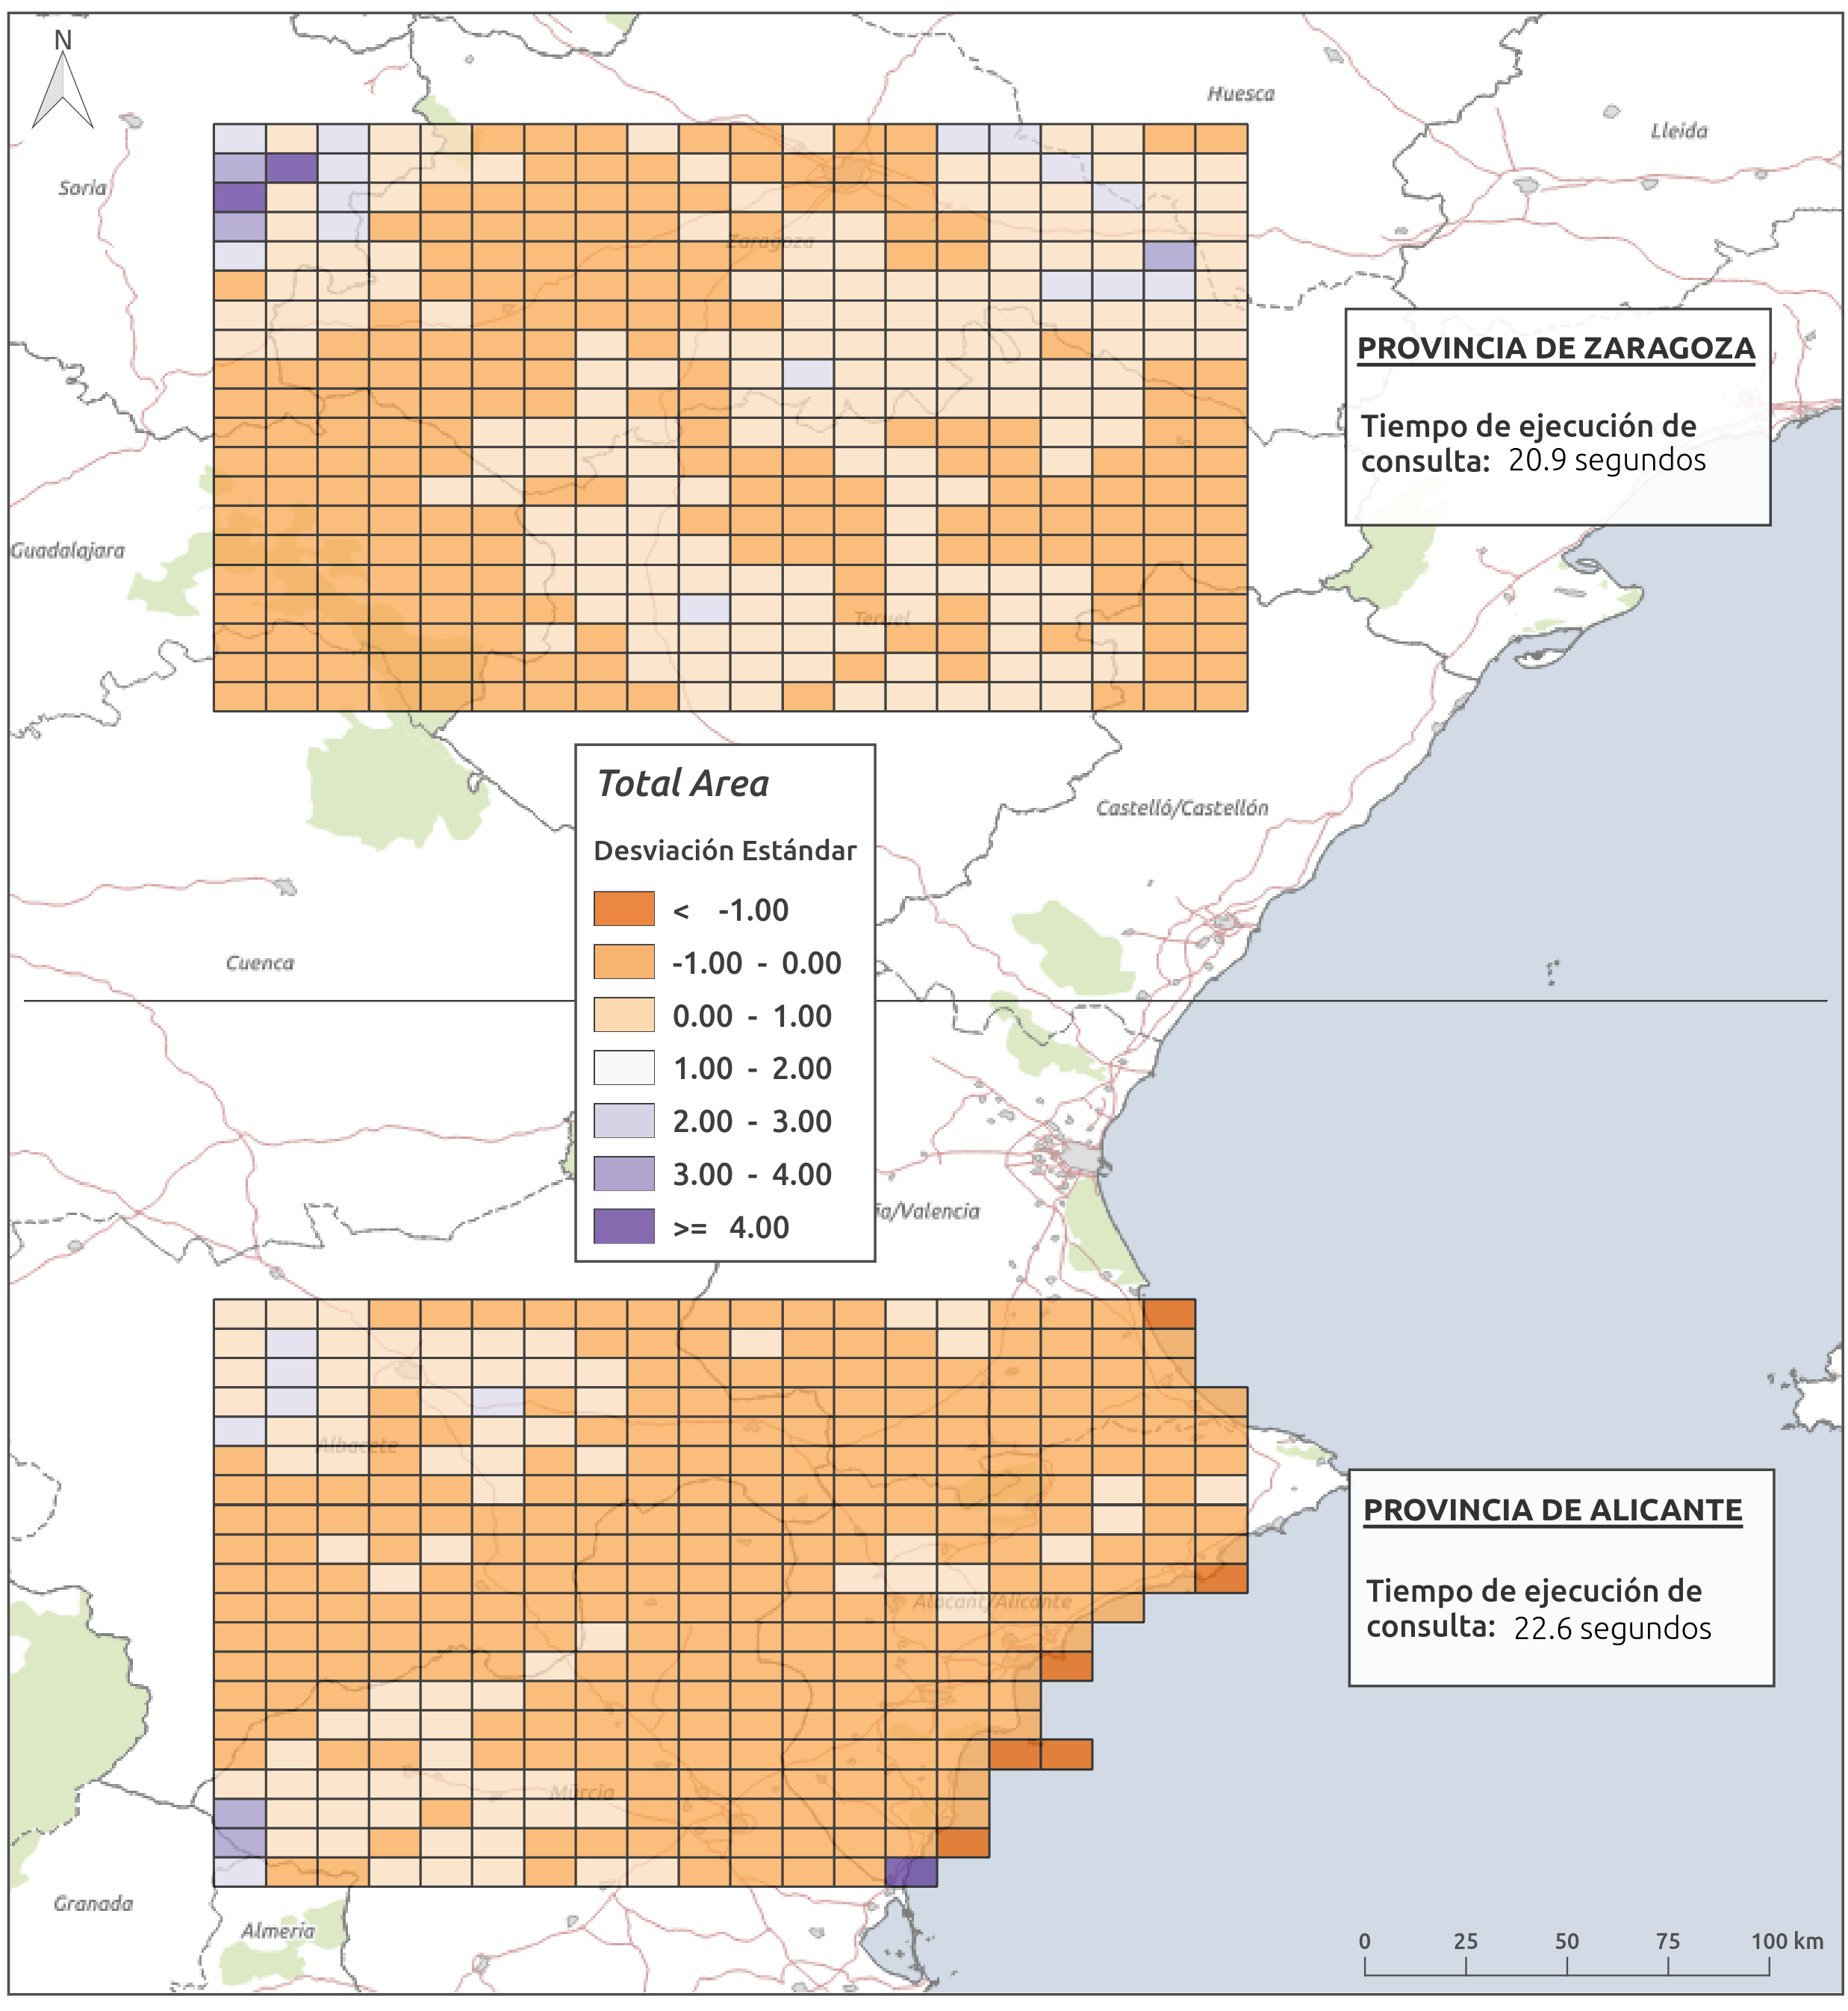
\includegraphics[width=\textwidth]{ResultadosyDiscusion/Figs/Results/l_25.png}
\caption{Título. \label{fig:l_25}}
\end{center}
\end{figure}

\begin{figure}
\begin{center}
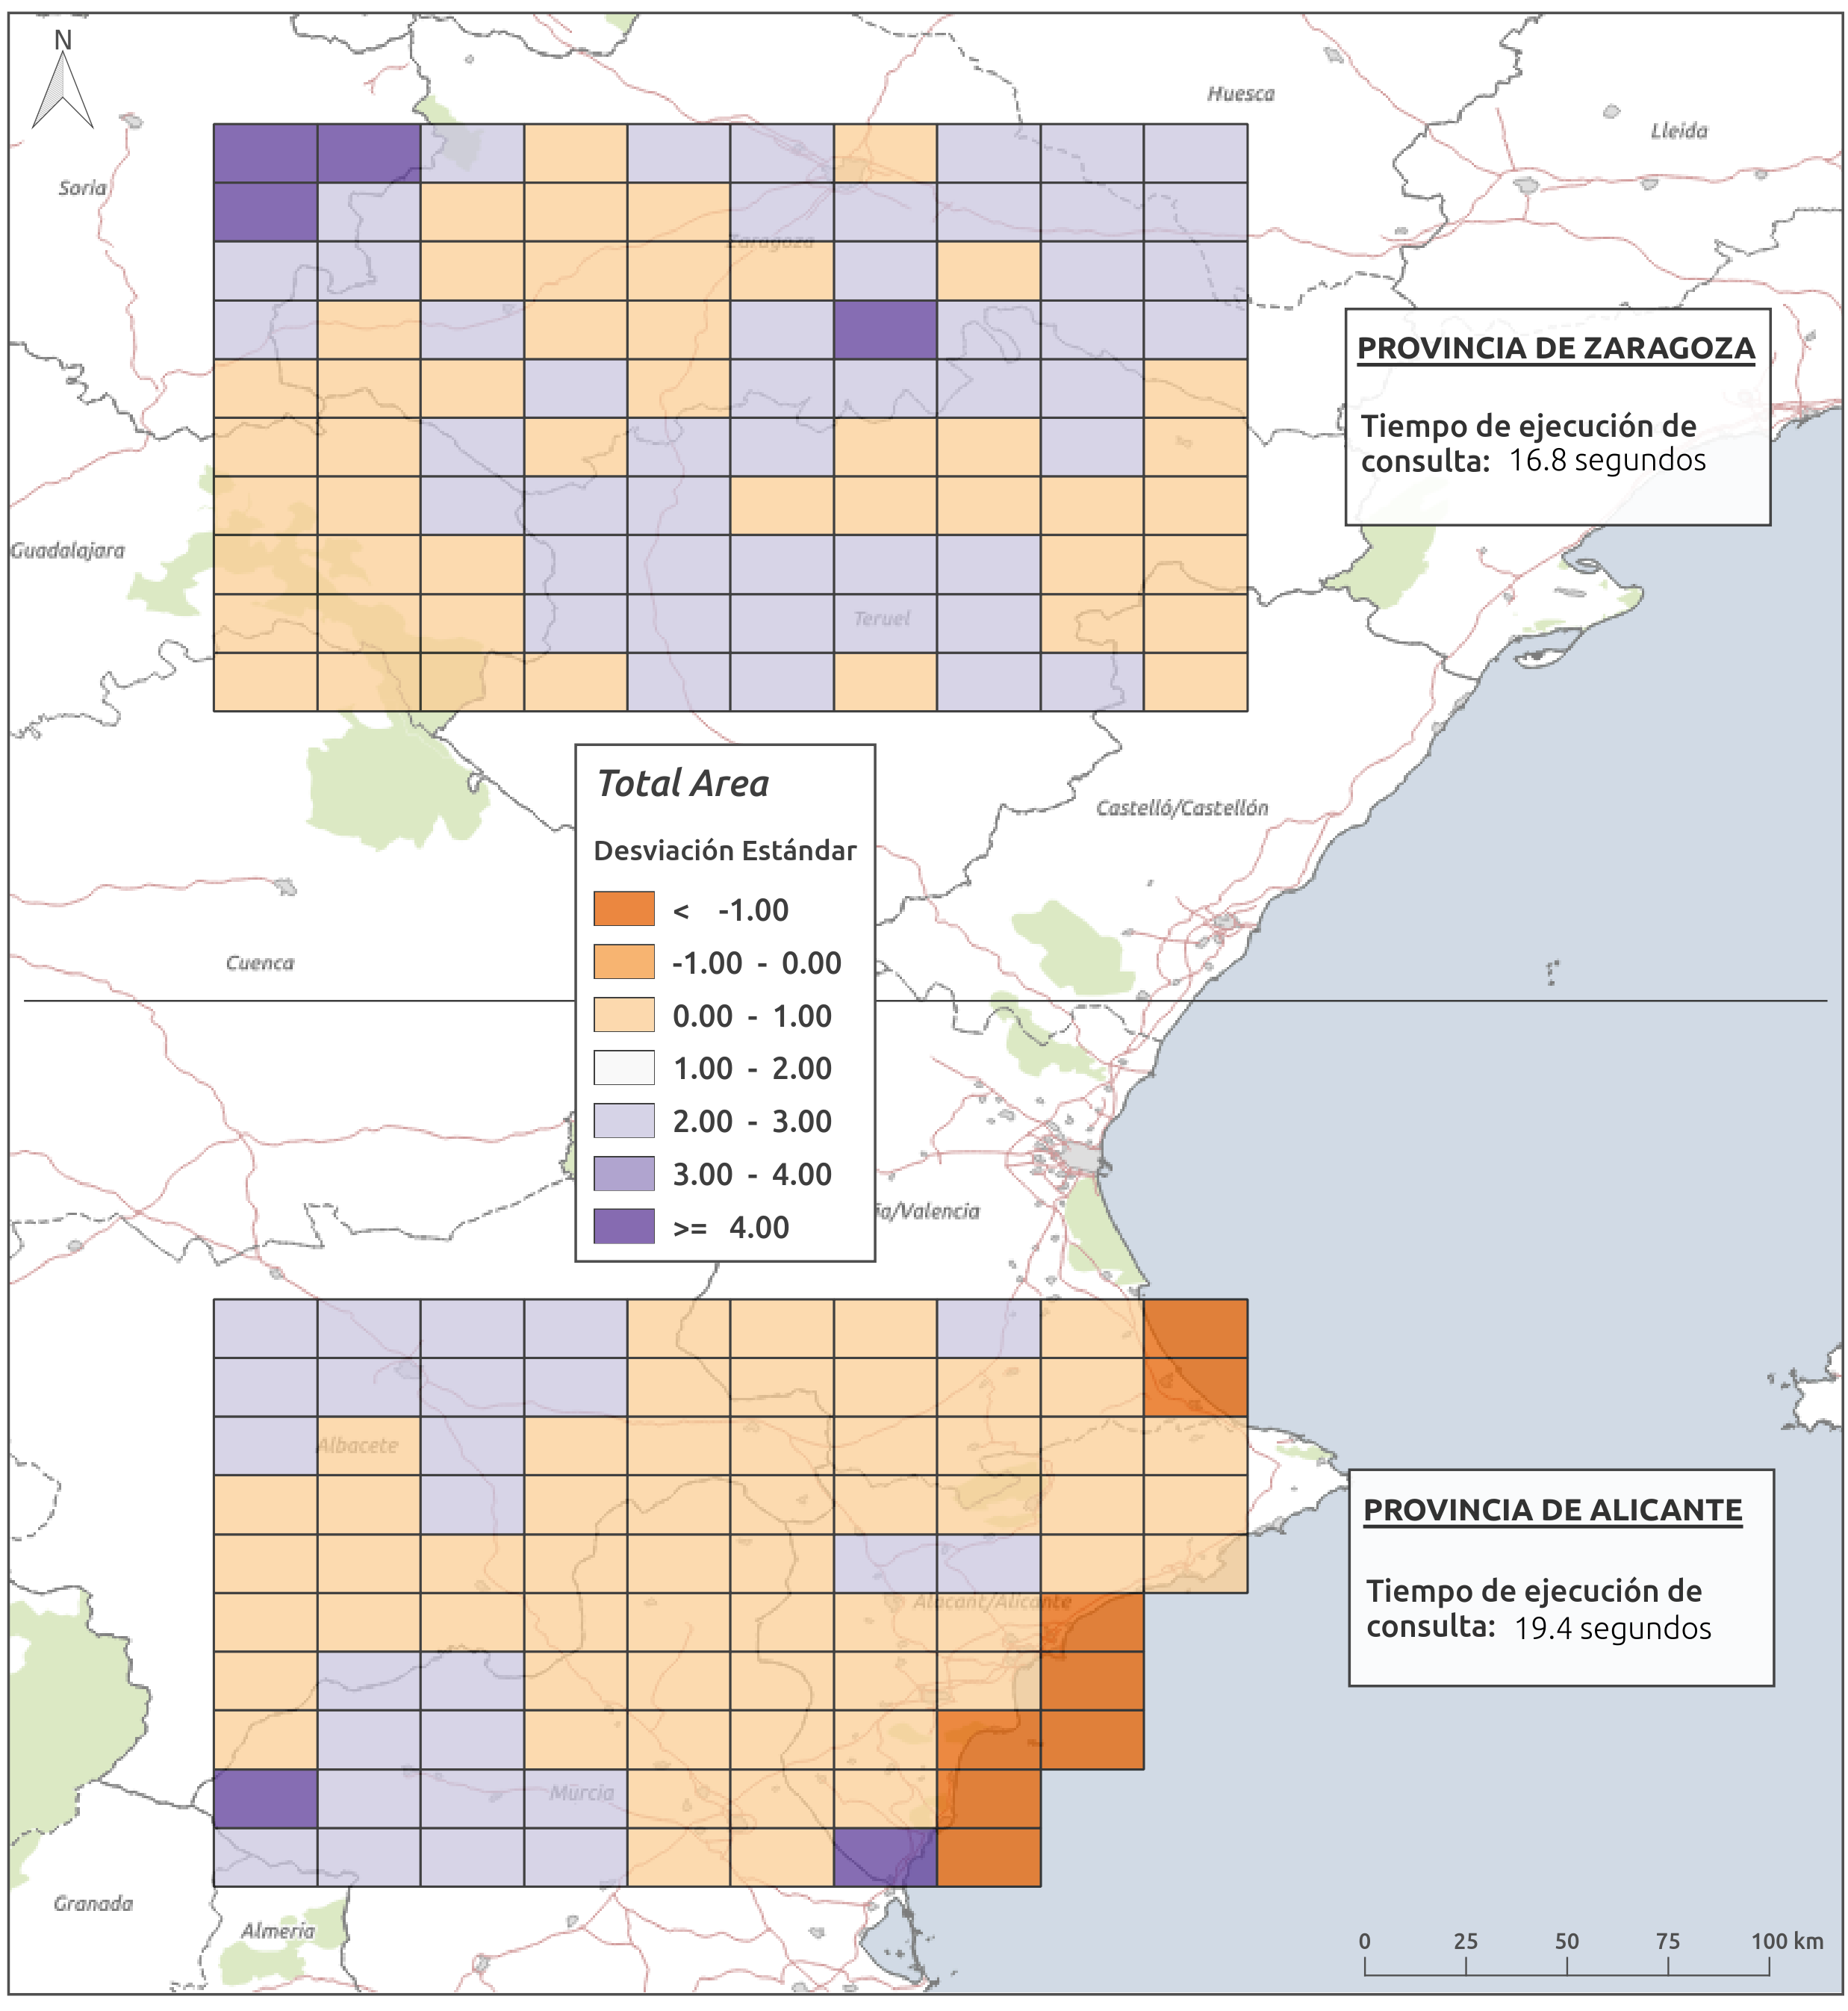
\includegraphics[width=\textwidth]{ResultadosyDiscusion/Figs/Results/l_50.png}
\caption{Título. \label{fig:l_50}}
\end{center}
\end{figure}

\begin{figure}
\begin{center}
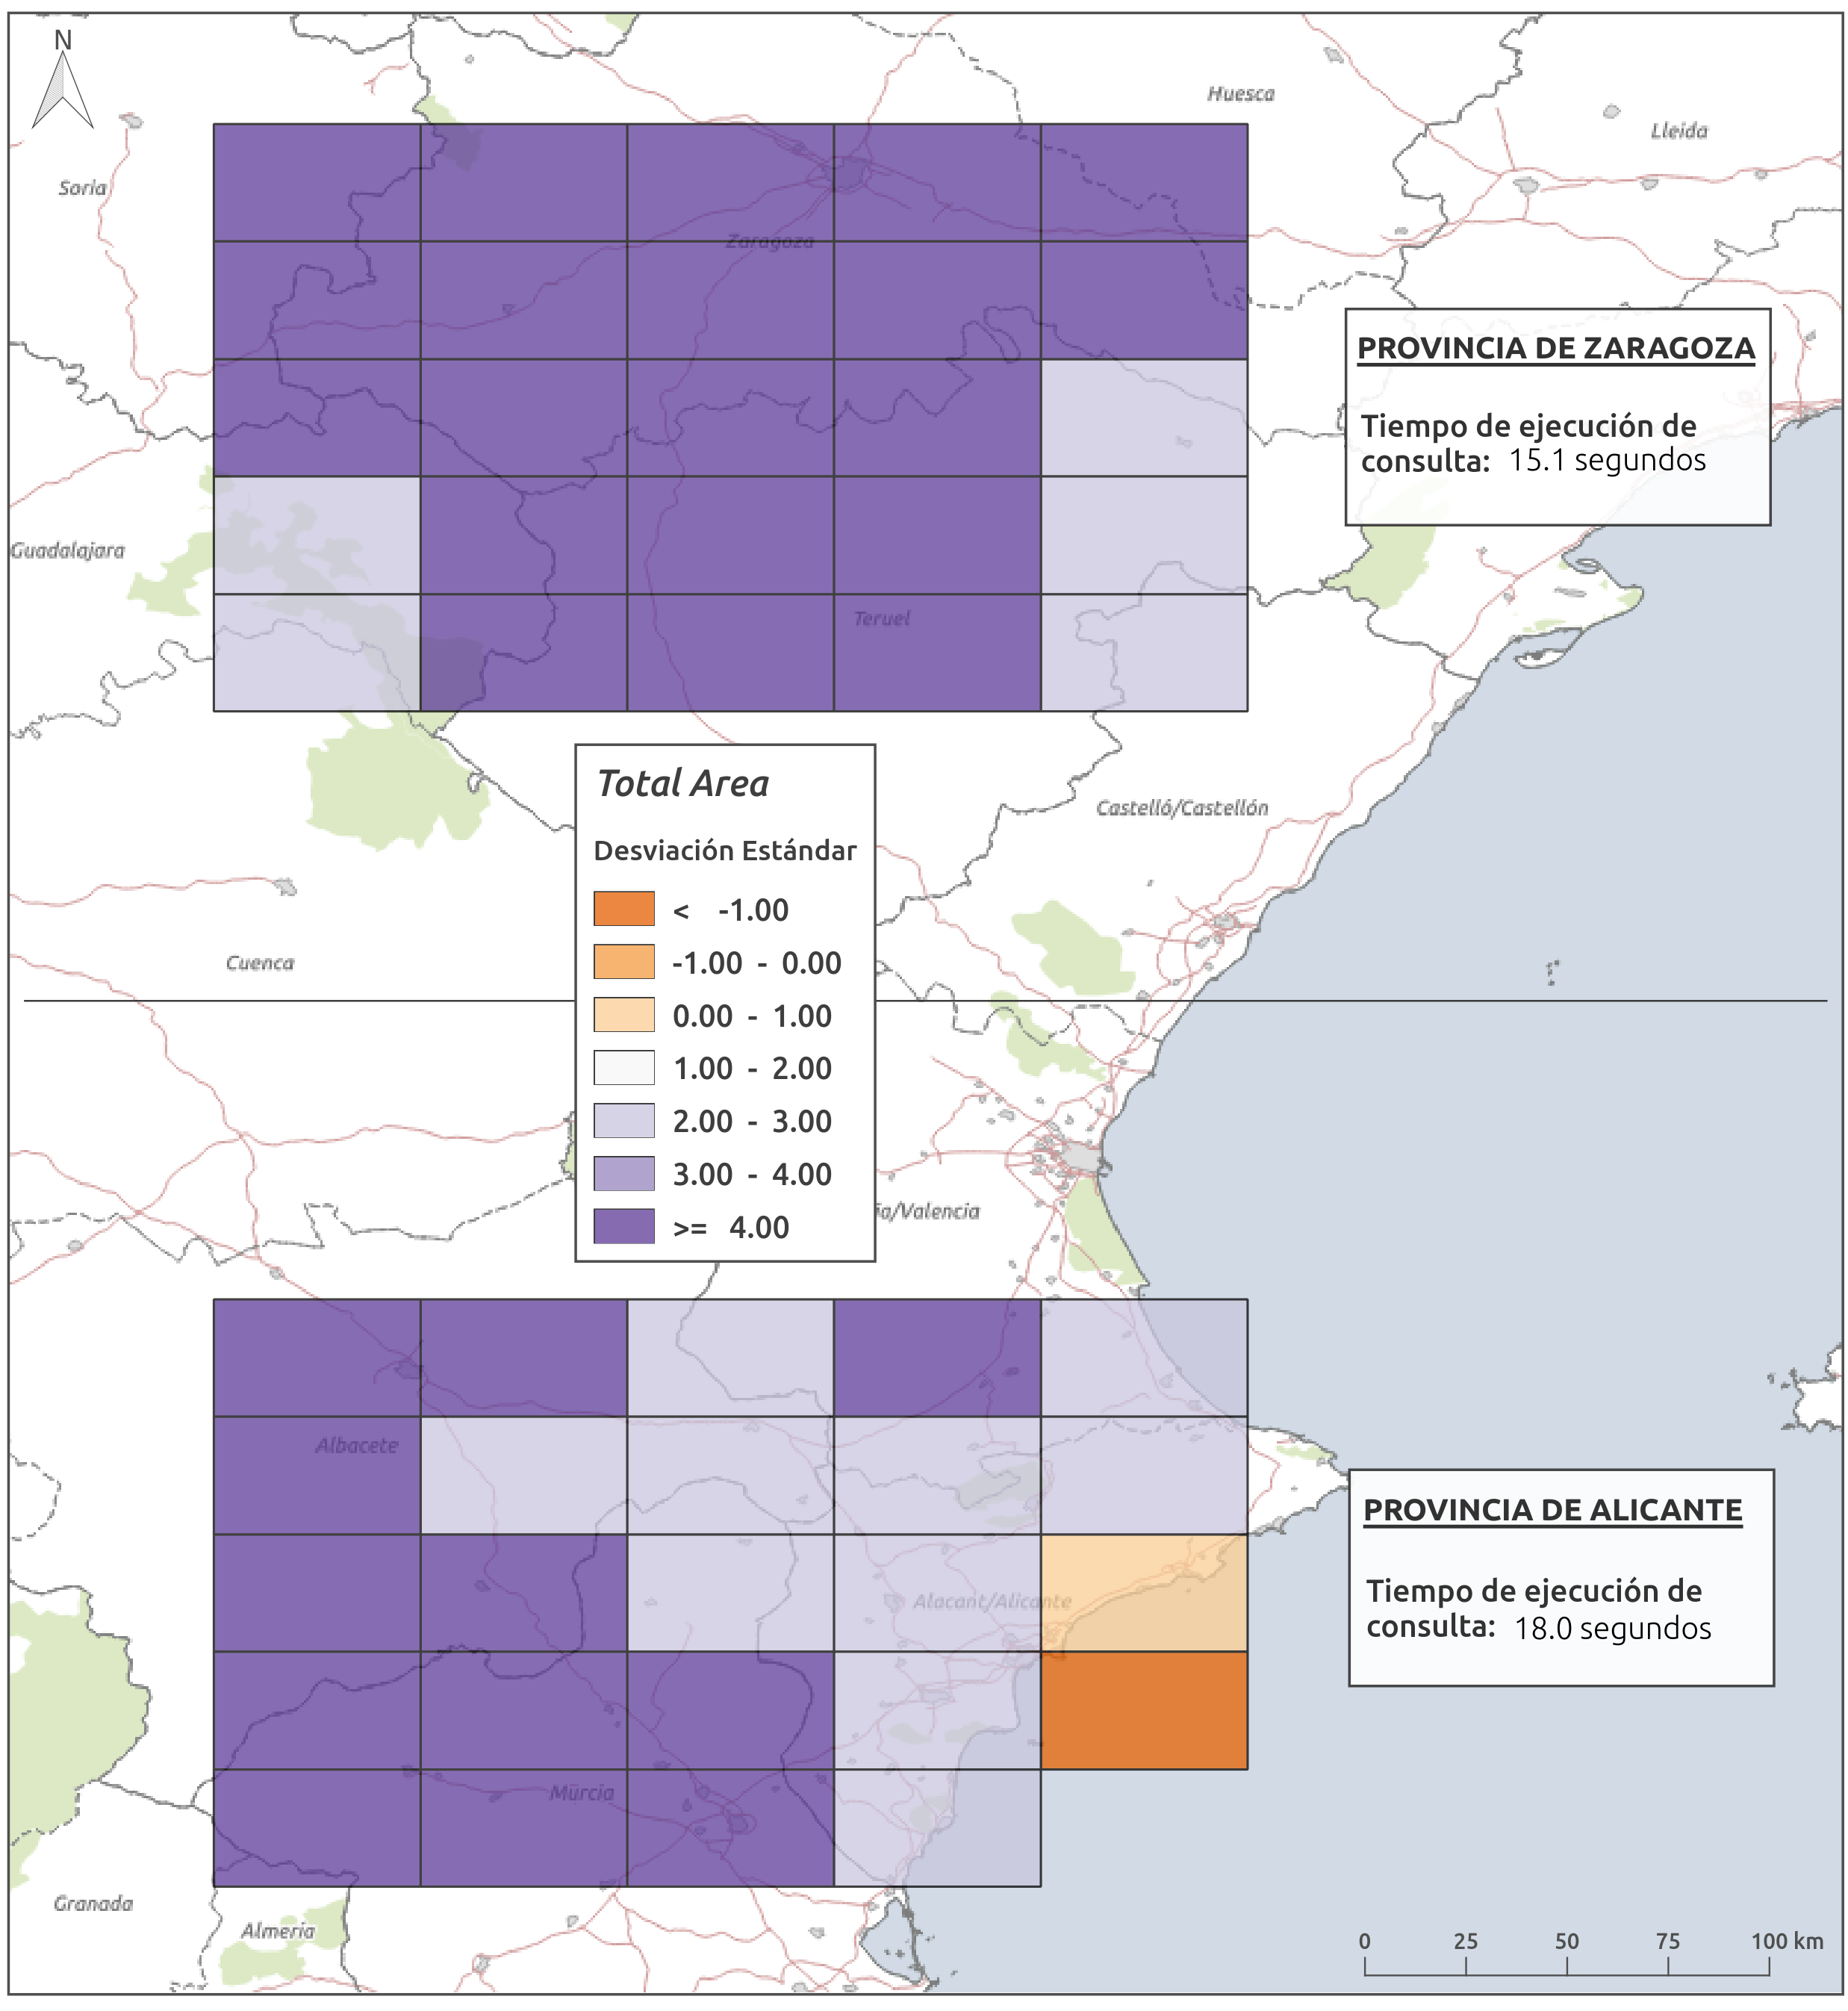
\includegraphics[width=\textwidth]{ResultadosyDiscusion/Figs/Results/l_100.png}
\caption{Título. \label{fig:l_100}}
\end{center}
\end{figure}